\suppnote{Supplementary Note S16. Strict-gate failure diagnostics}\label{si:v4-stage1}
The offline analysis reuses the retained V3 records. All six strict-gate failures remain in the denominator of 120 strict attempts. The ungated and moderate conditions each retain 120 attempts. Twenty-one trajectories include the six failures, their twelve matched ungated and moderate runs, and three strict successes chosen by a fixed identity hash within the failed model, representation, and prompt strata.

The complete tables and pinned-tokenizer text windows are retained under \path{results/revision_v4/source_tables}. The accompanying manifest records every raw input hash and the selection rules. These trajectories describe the capacity accounting and observed local contexts. They do not establish a causal linguistic explanation. The local windows below show public-service lists, project-update formatting and a repeated CRM-budget closing, among other contexts. These are observed associations. Low entropy also occurs in the selected successful trajectories, so these textual patterns are not established causes. The retained runs used no token filter and sampled ordinary skips with temperature 0.8 and top-p 0.95. They were not greedy-skip experiments.

At the fixed maximum budget \(T=6L\), completion requires at least \(L\) eligible positions, so a failure has \(\sum_{t=1}^{T}\mathbf{1}\{H_t\geq\tau\}<L\). The six observed eligible fractions range from 0.0768 to 0.1510, all below \(1/6\). The ordinary-development 75th percentile does not guarantee a 25\% eligibility rate on later payload-conditioned trajectories. Long below-threshold stretches explain the recorded lack of rank progress mechanically, while the text windows alone cannot identify a linguistic cause.

\begin{table}[H]
\centering\small
\begin{tabular}{lrrrrr}
\toprule
Trial suffix & Requested & Consumed & Budget & Longest run & Eligible fraction \\
\midrule
56249891 & 128 & 110 & 768 & 50 & 0.1432 \\
8a26bf09 & 128 & 116 & 768 & 163 & 0.1510 \\
c8241d5a & 64 & 54 & 384 & 39 & 0.1406 \\
fa8be8b1 & 128 & 106 & 768 & 35 & 0.1380 \\
fbecb170 & 128 & 59 & 768 & 267 & 0.0768 \\
1fbd18ec & 128 & 116 & 768 & 51 & 0.1510 \\
\bottomrule
\end{tabular}
\caption{All six retained strict-gate completion failures. Longest run counts consecutive positions below threshold. Full identities and exact half-open ranges are in the accompanying CSV.}\label{tab:v4-failures}
\end{table}

\begin{figure}[H]
\centering
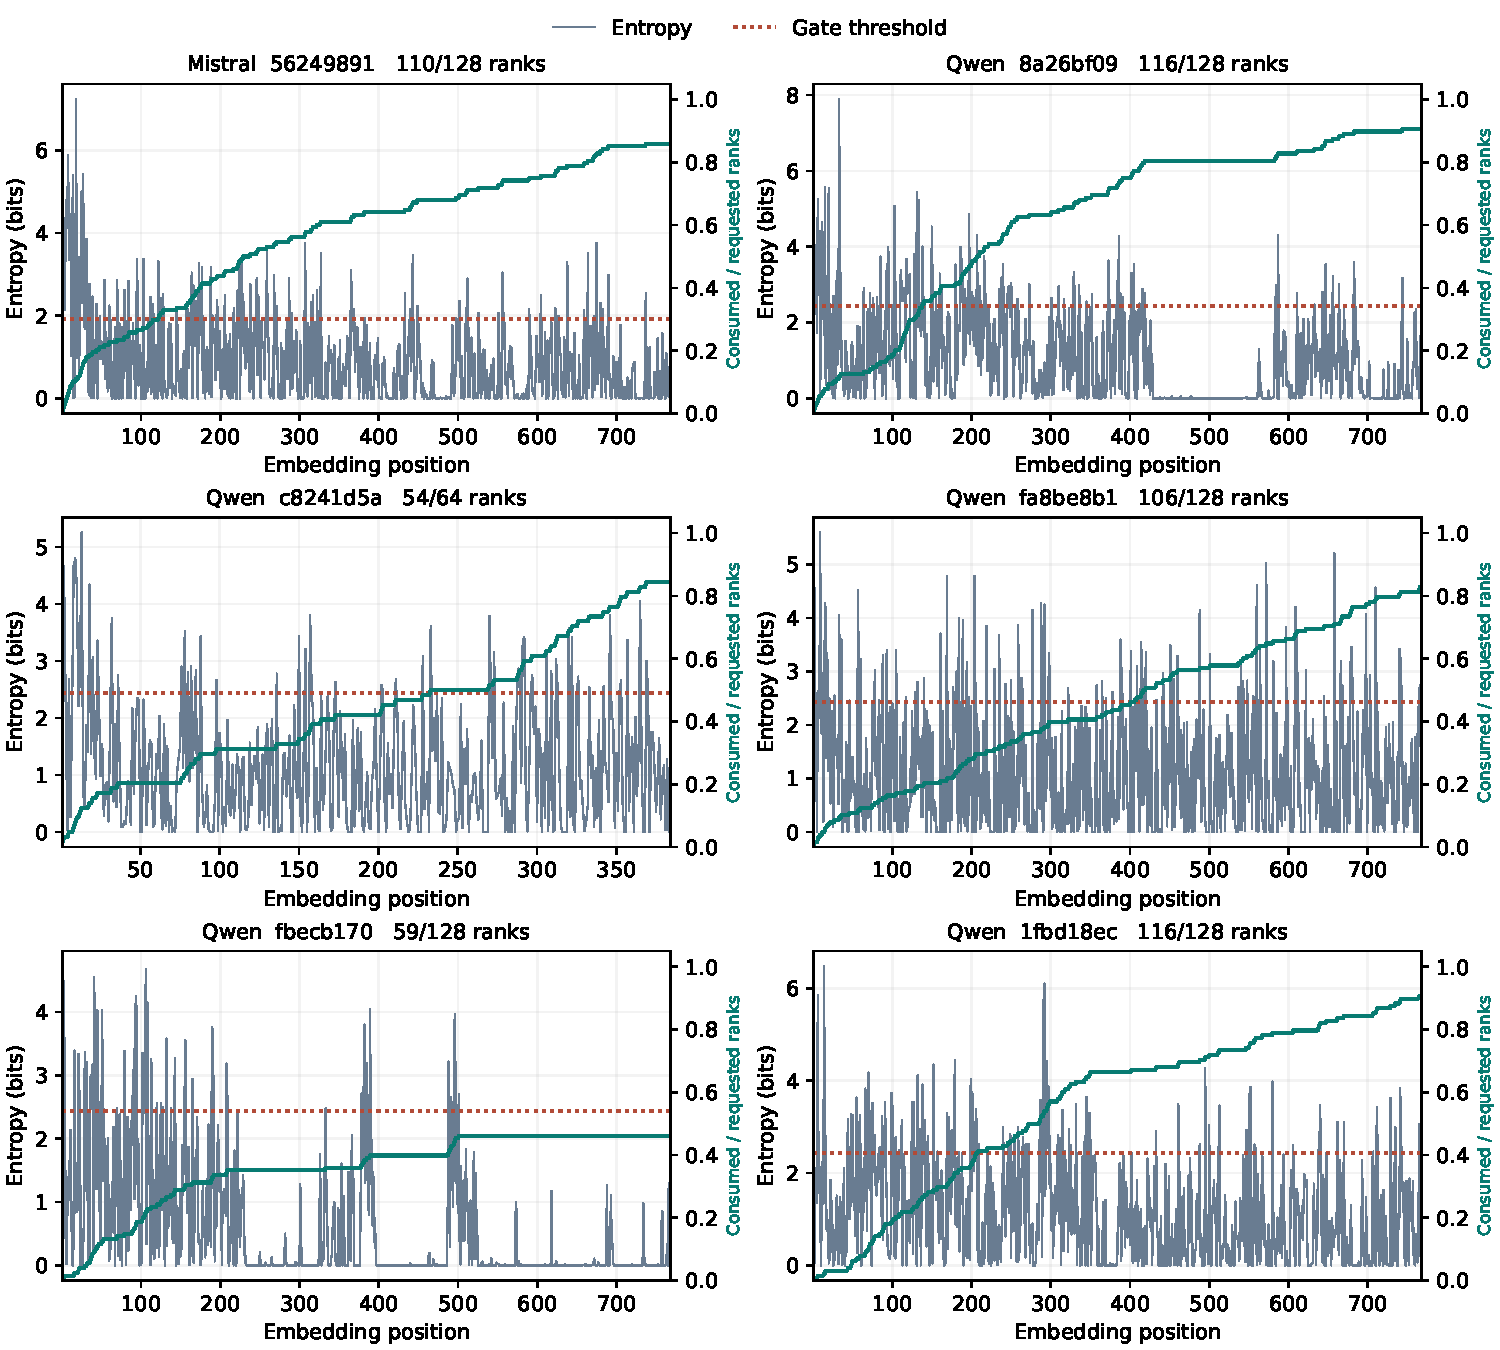
\includegraphics[width=\textwidth]{figures/v4_entropy_failure_traces.pdf}
\caption{Existing strict-gate failure trajectories. Entropy is measured before each token and compared with the frozen model threshold. Cumulative consumed ranks are normalized by the requested count. All six trajectories exhaust their token budgets before completion. This is exploratory evidence from retained records.}\label{fig:v4-entropy}
\end{figure}
